%%%%%%%%%%%%%%%%%%%%%%%%%%%%%%%%%%%%%%%%%%%%%%%%%%%%%%%%%%%%%%%%%%%%%%%%%%%%%%%%%%%%%%%%%%%%%
%%									Chapitre 1											%
%%%%%%%%%%%%%%%%%%%%%%%%%%%%%%%%%%%%%%%%%%%%%%%%%%%%%%%%%%%%%%%%%%%%%%%%%%%%%%%%%%%%%%%%%%%%%
\chapter{An Overview of the Thesis}\label{chap:intro}
	\citationChap{
	The thing about quotes on the internet is that you can not confirm their validity
	}{Abraham Lincoln}
	\minitoc
	\newpage

%%%%%%%%%%%%%%%%%%%%%%%%%%%%%%%%%%%%%%%%%%%%%%%%%%%%%%%%%%%%%%%%%%%%%%%%%%%%%%%%%%%%%%%%%%%%%



% Début du chapitre

The purpose of this dissertation is to make  of the majority of my research work carried out in between October 2017 and March 2021. My research took place at the IETR laboratory in Rennes (France), in the SCEE team, hosted on the Rennes campus of the engineering school CentraleSupélec. I was supervised by Professor Christophe Moy, in Rennes, and I was also co-supervised by Doctor Émilie Kaufmann, whom I visited many times at Inria Lille Nord Europe in Lille (France).

\section{Context of the Thesis}\label{sec:intro.context}
	
\subsection{What do we study and why?}\label{sec:intro.context.what}
	    
	\gls{mab}

% 	\begin{tableth}
% 		\caption[Légende courte pour l'exemple de tableau]{Un tableau avec une légende tellement longue que ce serait hideux dans la liste des tableaux}
% 			\label{tab:exemple}
% 		\begin{tabular}{c|c}
% 			Coucou	& Au revoir\\
% 			\hline
% 			maman	& papa
% 		\end{tabular}
% 	\end{tableth}

% 	\begin{figureth}
% 		\begin{subfigureth}{0.4\textwidth}
% 			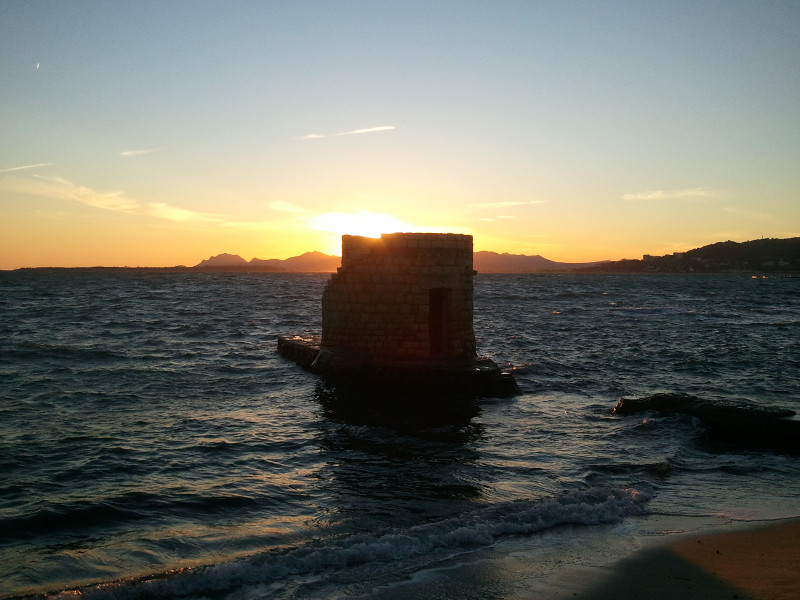
\includegraphics[width=\linewidth]{Chapter1/img/Antibes}
% 			\caption{Photo du Cap d'Antibes}
% 				\label{sub:Antibes}
% 		\end{subfigureth}
% 		\begin{subfigureth}{0.4\textwidth}
% 			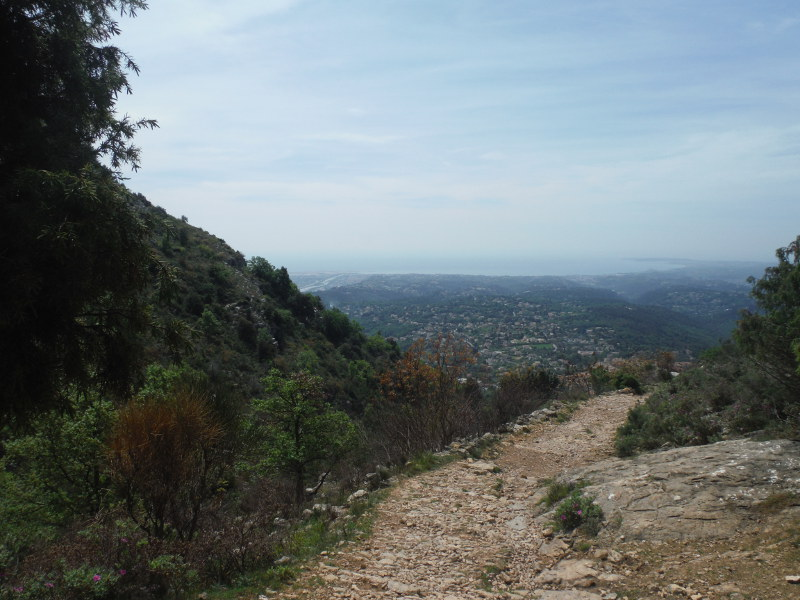
\includegraphics[width=\linewidth]{Chapter1/img/SaintJeannet}
% 			\caption{Saint Jeannet, depuis son Baou}
% 				\label{sub:SaintJeannet}
% 		\end{subfigureth}
% 		\caption[Légende courte pour la figure]{Exemple d'utilisation des sous-figures. J'utilise ici volontairement une légende longue.}
% 			\label{fig:exemple}
% 	\end{figureth}

\section{Multi-Armed Bandits and Optimization}\label{sec:intro.mab}
    
My previous research tries to address sequential optimisation problems under stochastic environments. A stochastic environment refers to an environment from which stochastic feedback are acquired when a data point is queried from the search/action space $\mathcal{X}$. Formally, we aim to maximise a target function $f:\mathcal{X}\rightarrow\mathbb{R}$, i.e. find 
\begin{equation}\label{eq:optim}
    \argmax_{x\in\mathcal{X}} f(x)\,.
\end{equation}

In its simplest form where the action space $\mathcal{X}$ is finite, the problem can be modeled as a \emph{stochastic multi-armed bandit}. The term \emph{bandit} is named, by analogy, after slot machines (or one-armed bandits) in a casino. A \emph{sequential decision making} problem comes up then when facing with several slot machines (multi-armed bandits). Concretely, a stochastic bandit is a collection of $K$ actions (also called arms) $\mathcal{X} = \{x_1,\ldots,x_K\}$. Each time the learner chooses one action $x_{a_t}\in\mathcal{X}$ which is then fed to the environment. The environment generates a reward $r_{a_t,t}=r_t$ which is assumed to be drawn from an unknown $[0,1]$-valued distribution $\nu_{a_t}$ and is revealed to the learner.

In its original formulation, the learning objective of a stochastic bandit is to maximise the total reward $\sum_{t=1}^T r_t$ obtained within a given time horizon $T$. In the literature of bandit, we usually denote by $\mu_k$ (resp. $\mu^\star$) the expectation of the unknown distribution $\nu_k$ (resp. the optimal arm), and the previous reward maximisation objective is equivalent to minimising the \emph{cumulative regret}: $T\mu^\star-\sum_{t=1}^T \mu_{a_t}$. %A such learning objective requires the learner to simultaneously acquire new information for potential future well-being (called \emph{exploration}), and optimize the current decision based on past observations (called \emph{exploitation}). 
Multi-armed bandits naturally addresses the trade-off between exploration and exploitation.

My PhD work, on the other hand, focuses on another learning objective which aims at identifying the optimal action, namely \emph{best-arm identification} (BAI). Contrary to regret minimisation, best-arm identification only cares about the exploration. Note that in this case, the time horizon $T$ is not necessarily known to the learner: we are often interested in finding the best arm with a given confidence level with as few queries as possible since in real applications function evaluations could be very expensive. This problem possesses many interesting variants and extensions that can all be formulated as the optimisation problem~\eqref{eq:optim} to some extent, some of which will be covered in the next as I briefly describe some of the main contributions of my thesis.
    
    
\section{A Summary of the Contributions}\label{sec:intro.contributions}

\paragraph{Bayesian best-arm identification.} We begin by the vanilla BAI, for which the search space $\mathcal{X}$ is finite and one-dimensional and the target function $f$ can be considered as a function that maps each arm $x_k$ to its mean $\mu_k$. In one of our papers~\citep{shang2020t3c}, we employ some Bayesian machinery to address the problem based on the famous Thompson sampling (\TS). \TS is a Bayesian algorithm well known for regret minimization, for which it is now seen as a major competitor to the popular \UCB-typed approaches~\citep{auer2002ucb}. A natural question to ask is whether Bayesian methods can be also a good competitor to classical BAI approaches constructed upon complicated confidence intervals. However, it is well known that direct use of \TS cannot yield optimal performance for BAI and an adaptation such as \TTTS (top-two Thompson sampling) proposed by~\cite{russo2016ttts} is needed: by choosing between two different candidate arms in each round, it enforces the exploration of sub-optimal arms, which would be under-sampled by vanilla \TS due to its objective of maximizing rewards. \cite{shang2020t3c} provides further theoretical understandings of \TTTS and proposes a computational improvement \TCC with the same guarantees. \cite{shang2019dttts} also show that with some minor modifications, such Bayesian-flavored algorithms can be good candidates for applications like hyper-parameter optimisation.

\paragraph{Extension to pure exploration for linear bandits.} A very natural and popular extension of the vanilla BAI is to take a finite space of features $\cX$ in $\R^d$ as the search space and consider a target function $f$ that maps each arm $\mathbf{x}$ (also called context in this case) to its linear combination with a \emph{regression parameter} $\btheta$, and is thus called linear bandits. $\btheta$ is of course unknown to the learner. Previous work on this topic were not (asymptotically) optimal. A lower bound, which can be written as a complicated minimax optimisation problem, is given by~\cite{garivier2016tracknstop}. In a subsequent work, we develop a saddle-point approach to that lower bound optimisation problem, which then led to optimal algorithms for linear BAI in the fixed-confidence regime~\citep{degenne2020game}. In addition, their empirical performance is competitive with the best existing algorithms. We also investigate a natural adaptation of our Bayesian approaches developed in the previous paper~\citep{shang2020t3c}. Unfortunately, they do not seem to be (asymptotically) optimal (work not published yet). Therefore, knowing whether one can find an *optimal* Bayesian approach remains an open problem.

\paragraph{Infinitely-armed bandits and black-box optimisation.} Finally, a more general problem is to consider an infinite (probably uncountable) measurable space $\mathcal{X}$, and each arm $x\in\mathcal{X}$ gets its mean reward $f(x)$ through the reward function $f$. We study the noisy setting in which the obtained reward is a noisy evaluation of $f: r_t = f(x_t) + \epsilon_t$. This problem is also better known under the name \emph{black-box optimisation}, to which the main approaches include Bayesian optimisation~\citep{brochu2010bayesian}, evolutionary algorithms and hierarchical bandits~\citep{bubeck2010x}. We opt for another performance measure in this case, namely the simple regret: $\max_{x\in\mathcal{X}} f(x) - f(x_{j_t})$ with $x_{j_t}$ our guess at time $t$. In a recent work of ours, we provide a general wrapper for hierarchical bandit algorithms that only have guarantees for their simple regret~\cite{shang2019adaptive}. We show that with a cross-validation scheme, any hierarchical bandit algorithm with simple regret guarantees can be plugged into our meta-algorithm with only a tiny increase in the resulting simple regret.

\paragraph{Included in this thesis}

\cite{shang2018adaptive,shang2019dttts,shang2019adaptive,shang2020dttts,degenne2020game,shang2020t3c}.

\paragraph{Not included in this thesis}

\cite{shang2020vector,shang2021safe,menard2021ucbmq}.

\cite{rlberry2021}.

\section{Organization of the Thesis}\label{sec:intro.organization}

% \newpage
% \bibliographystyle{plain}
% \bibliography{library}
